
%% bare_conf.tex
%% V1.4b
%% 2015/08/26
%% by Michael Shell
%% See:
%% http://www.michaelshell.org/
%% for current contact information.
%%
%% This is a skeleton file demonstrating the use of IEEEtran.cls
%% (requires IEEEtran.cls version 1.8b or later) with an IEEE
%% conference paper.
%%
%% Support sites:
%% http://www.michaelshell.org/tex/ieeetran/
%% http://www.ctan.org/pkg/ieeetran
%% and
%% http://www.ieee.org/

%%*************************************************************************
%% Legal Notice:
%% This code is offered as-is without any warranty either expressed or
%% implied; without even the implied warranty of MERCHANTABILITY or
%% FITNESS FOR A PARTICULAR PURPOSE! 
%% User assumes all risk.
%% In no event shall the IEEE or any contributor to this code be liable for
%% any damages or losses, including, but not limited to, incidental,
%% consequential, or any other damages, resulting from the use or misuse
%% of any information contained here.
%%
%% All comments are the opinions of their respective authors and are not
%% necessarily endorsed by the IEEE.
%%
%% This work is distributed under the LaTeX Project Public License (LPPL)
%% ( http://www.latex-project.org/ ) version 1.3, and may be freely used,
%% distributed and modified. A copy of the LPPL, version 1.3, is included
%% in the base LaTeX documentation of all distributions of LaTeX released
%% 2003/12/01 or later.
%% Retain all contribution notices and credits.
%% ** Modified files should be clearly indicated as such, including  **
%% ** renaming them and changing author support contact information. **
%%*************************************************************************


% *** Authors should verify (and, if needed, correct) their LaTeX system  ***
% *** with the testflow diagnostic prior to trusting their LaTeX platform ***
% *** with production work. The IEEE's font choices and paper sizes can   ***
% *** trigger bugs that do not appear when using other class files.       ***                          ***
% The testflow support page is at:
% http://www.michaelshell.org/tex/testflow/



\documentclass[conference]{IEEEtran}
\usepackage{multirow}
% Some Computer Society conferences also require the compsoc mode option,
% but others use the standard conference format.
%
% If IEEEtran.cls has not been installed into the LaTeX system files,
% manually specify the path to it like:
% \documentclass[conference]{../sty/IEEEtran}





% Some very useful LaTeX packages include:
% (uncomment the ones you want to load)


% *** MISC UTILITY PACKAGES ***
%
%\usepackage{ifpdf}
% Heiko Oberdiek's ifpdf.sty is very useful if you need conditional
% compilation based on whether the output is pdf or dvi.
% usage:
% \ifpdf
%   % pdf code
% \else
%   % dvi code
% \fi
% The latest version of ifpdf.sty can be obtained from:
% http://www.ctan.org/pkg/ifpdf
% Also, note that IEEEtran.cls V1.7 and later provides a builtin
% \ifCLASSINFOpdf conditional that works the same way.
% When switching from latex to pdflatex and vice-versa, the compiler may
% have to be run twice to clear warning/error messages.






% *** CITATION PACKAGES ***
%
%\usepackage{cite}
% cite.sty was written by Donald Arseneau
% V1.6 and later of IEEEtran pre-defines the format of the cite.sty package
% \cite{} output to follow that of the IEEE. Loading the cite package will
% result in citation numbers being automatically sorted and properly
% "compressed/ranged". e.g., [1], [9], [2], [7], [5], [6] without using
% cite.sty will become [1], [2], [5]--[7], [9] using cite.sty. cite.sty's
% \cite will automatically add leading space, if needed. Use cite.sty's
% noadjust option (cite.sty V3.8 and later) if you want to turn this off
% such as if a citation ever needs to be enclosed in parenthesis.
% cite.sty is already installed on most LaTeX systems. Be sure and use
% version 5.0 (2009-03-20) and later if using hyperref.sty.
% The latest version can be obtained at:
% http://www.ctan.org/pkg/cite
% The documentation is contained in the cite.sty file itself.






% *** GRAPHICS RELATED PACKAGES ***
%
\ifCLASSINFOpdf
  \usepackage[pdftex]{graphicx}

  % \usepackage[pdftex]{graphicx}
  % declare the path(s) where your graphic files are
  % \graphicspath{{../pdf/}{../jpeg/}}
  % and their extensions so you won't have to specify these with
  % every instance of \includegraphics
  % \DeclareGraphicsExtensions{.pdf,.jpeg,.png}
\else
  % or other class option (dvipsone, dvipdf, if not using dvips). graphicx
  % will default to the driver specified in the system graphics.cfg if no
  % driver is specified.
  % \usepackage[dvips]{graphicx}
  % declare the path(s) where your graphic files are
  % \graphicspath{{../eps/}}
  % and their extensions so you won't have to specify these with
  % every instance of \includegraphics
  % \DeclareGraphicsExtensions{.eps}
\fi
% graphicx was written by David Carlisle and Sebastian Rahtz. It is
% required if you want graphics, photos, etc. graphicx.sty is already
% installed on most LaTeX systems. The latest version and documentation
% can be obtained at: 
% http://www.ctan.org/pkg/graphicx
% Another good source of documentation is "Using Imported Graphics in
% LaTeX2e" by Keith Reckdahl which can be found at:
% http://www.ctan.org/pkg/epslatex
%
% latex, and pdflatex in dvi mode, support graphics in encapsulated
% postscript (.eps) format. pdflatex in pdf mode supports graphics
% in .pdf, .jpeg, .png and .mps (metapost) formats. Users should ensure
% that all non-photo figures use a vector format (.eps, .pdf, .mps) and
% not a bitmapped formats (.jpeg, .png). The IEEE frowns on bitmapped formats
% which can result in "jaggedy"/blurry rendering of lines and letters as
% well as large increases in file sizes.
%
% You can find documentation about the pdfTeX application at:
% http://www.tug.org/applications/pdftex





% *** MATH PACKAGES ***
%
\usepackage{amsmath}
%\usepackage{amsmath}
% A popular package from the American Mathematical Society that provides
% many useful and powerful commands for dealing with mathematics.
%
% Note that the amsmath package sets \interdisplaylinepenalty to 10000
% thus preventing page breaks from occurring within multiline equations. Use:
%\interdisplaylinepenalty=2500
% after loading amsmath to restore such page breaks as IEEEtran.cls normally
% does. amsmath.sty is already installed on most LaTeX systems. The latest
% version and documentation can be obtained at:
% http://www.ctan.org/pkg/amsmath





% *** SPECIALIZED LIST PACKAGES ***
%
%\usepackage{algorithmic}
% algorithmic.sty was written by Peter Williams and Rogerio Brito.
% This package provides an algorithmic environment fo describing algorithms.
% You can use the algorithmic environment in-text or within a figure
% environment to provide for a floating algorithm. Do NOT use the algorithm
% floating environment provided by algorithm.sty (by the same authors) or
% algorithm2e.sty (by Christophe Fiorio) as the IEEE does not use dedicated
% algorithm float types and packages that provide these will not provide
% correct IEEE style captions. The latest version and documentation of
% algorithmic.sty can be obtained at:
% http://www.ctan.org/pkg/algorithms
% Also of interest may be the (relatively newer and more customizable)
% algorithmicx.sty package by Szasz Janos:
% http://www.ctan.org/pkg/algorithmicx




% *** ALIGNMENT PACKAGES ***
%
%\usepackage{array}
% Frank Mittelbach's and David Carlisle's array.sty patches and improves
% the standard LaTeX2e array and tabular environments to provide better
% appearance and additional user controls. As the default LaTeX2e table
% generation code is lacking to the point of almost being broken with
% respect to the quality of the end results, all users are strongly
% advised to use an enhanced (at the very least that provided by array.sty)
% set of table tools. array.sty is already installed on most systems. The
% latest version and documentation can be obtained at:
% http://www.ctan.org/pkg/array


% IEEEtran contains the IEEEeqnarray family of commands that can be used to
% generate multiline equations as well as matrices, tables, etc., of high
% quality.




% *** SUBFIGURE PACKAGES ***
%\ifCLASSOPTIONcompsoc
%  \usepackage[caption=false,font=normalsize,labelfont=sf,textfont=sf]{subfig}
%\else
%  \usepackage[caption=false,font=footnotesize]{subfig}
%\fi
% subfig.sty, written by Steven Douglas Cochran, is the modern replacement
% for subfigure.sty, the latter of which is no longer maintained and is
% incompatible with some LaTeX packages including fixltx2e. However,
% subfig.sty requires and automatically loads Axel Sommerfeldt's caption.sty
% which will override IEEEtran.cls' handling of captions and this will result
% in non-IEEE style figure/table captions. To prevent this problem, be sure
% and invoke subfig.sty's "caption=false" package option (available since
% subfig.sty version 1.3, 2005/06/28) as this is will preserve IEEEtran.cls
% handling of captions.
% Note that the Computer Society format requires a larger sans serif font
% than the serif footnote size font used in traditional IEEE formatting
% and thus the need to invoke different subfig.sty package options depending
% on whether compsoc mode has been enabled.
%
% The latest version and documentation of subfig.sty can be obtained at:
% http://www.ctan.org/pkg/subfig




% *** FLOAT PACKAGES ***
%
%\usepackage{fixltx2e}
% fixltx2e, the successor to the earlier fix2col.sty, was written by
% Frank Mittelbach and David Carlisle. This package corrects a few problems
% in the LaTeX2e kernel, the most notable of which is that in current
% LaTeX2e releases, the ordering of single and double column floats is not
% guaranteed to be preserved. Thus, an unpatched LaTeX2e can allow a
% single column figure to be placed prior to an earlier double column
% figure.
% Be aware that LaTeX2e kernels dated 2015 and later have fixltx2e.sty's
% corrections already built into the system in which case a warning will
% be issued if an attempt is made to load fixltx2e.sty as it is no longer
% needed.
% The latest version and documentation can be found at:
% http://www.ctan.org/pkg/fixltx2e


%\usepackage{stfloats}
% stfloats.sty was written by Sigitas Tolusis. This package gives LaTeX2e
% the ability to do double column floats at the bottom of the page as well
% as the top. (e.g., "\begin{figure*}[!b]" is not normally possible in
% LaTeX2e). It also provides a command:
%\fnbelowfloat
% to enable the placement of footnotes below bottom floats (the standard
% LaTeX2e kernel puts them above bottom floats). This is an invasive package
% which rewrites many portions of the LaTeX2e float routines. It may not work
% with other packages that modify the LaTeX2e float routines. The latest
% version and documentation can be obtained at:
% http://www.ctan.org/pkg/stfloats
% Do not use the stfloats baselinefloat ability as the IEEE does not allow
% \baselineskip to stretch. Authors submitting work to the IEEE should note
% that the IEEE rarely uses double column equations and that authors should try
% to avoid such use. Do not be tempted to use the cuted.sty or midfloat.sty
% packages (also by Sigitas Tolusis) as the IEEE does not format its papers in
% such ways.
% Do not attempt to use stfloats with fixltx2e as they are incompatible.
% Instead, use Morten Hogholm'a dblfloatfix which combines the features
% of both fixltx2e and stfloats:
%
% \usepackage{dblfloatfix}
% The latest version can be found at:
% http://www.ctan.org/pkg/dblfloatfix




% *** PDF, URL AND HYPERLINK PACKAGES ***
%
%\usepackage{url}
% url.sty was written by Donald Arseneau. It provides better support for
% handling and breaking URLs. url.sty is already installed on most LaTeX
% systems. The latest version and documentation can be obtained at:
% http://www.ctan.org/pkg/url
% Basically, \url{my_url_here}.




% *** Do not adjust lengths that control margins, column widths, etc. ***
% *** Do not use packages that alter fonts (such as pslatex).         ***
% There should be no need to do such things with IEEEtran.cls V1.6 and later.
% (Unless specifically asked to do so by the journal or conference you plan
% to submit to, of course. )


% correct bad hyphenation here
\hyphenation{op-tical net-works semi-conduc-tor}


\begin{document}
%

% paper title
% Titles are generally capitalized except for words such as a, an, and, as,
% at, but, by, for, in, nor, of, on, or, the, to and up, which are usually
% not capitalized unless they are the first or last word of the title.
% Linebreaks \\ can be used within to get better formatting as desired.
% Do not put math or special symbols in the title.
\title{A Multi-view Auto Lip-reading\\ The Kip-reasder's (Final Report)}


% author names and affiliations
% use a multiple column layout for up to three different
% affiliations
\author{%
\IEEEauthorblockN{Houjeung Han}
\IEEEauthorblockA{School of Electrical Engineering\\
KAIST\\
Daejeon, Korea\\
Email: comc35@kaist.ac.kr}%
\and
\IEEEauthorblockN{Jesper Loenbaek}
\IEEEauthorblockA{School of Computing\\
KAIST\\
Daejeon, Korea\\
Email: lonbak@kaist.ac.kr}%
\and
\IEEEauthorblockN{Youngsoo Jang}
\IEEEauthorblockA{School of Computing\\
KAIST\\
Daejeon, Korea\\
Email: jys5609@kaist.ac.kr}%
}

% conference papers do not typically use \thanks and this command
% is locked out in conference mode. If really needed, such as for
% the acknowledgment of grants, issue a \IEEEoverridecommandlockouts
% after \documentclass

% for over three affiliations, or if they all won't fit within the width
% of the page, use this alternative format:
% 
%\author{\IEEEauthorblockN{Michael Shell\IEEEauthorrefmark{1},
%Homer Simpson\IEEEauthorrefmark{2},
%James Kirk\IEEEauthorrefmark{3}, 
%Montgomery Scott\IEEEauthorrefmark{3} and
%Eldon Tyrell\IEEEauthorrefmark{4}}
%\IEEEauthorblockA{\IEEEauthorrefmark{1}School of Electrical and Computer Engineering\\
%Georgia Institute of Technology,
%Atlanta, Georgia 30332--0250\\ Email: see http://www.michaelshell.org/contact.html}
%\IEEEauthorblockA{\IEEEauthorrefmark{2}Twentieth Century Fox, Springfield, USA\\
%Email: homer@thesimpsons.com}
%\IEEEauthorblockA{\IEEEauthorrefmark{3}Starfleet Academy, San Francisco, California 96678-2391\\
%Telephone: (800) 555--1212, Fax: (888) 555--1212}
%\IEEEauthorblockA{\IEEEauthorrefmark{4}Tyrell Inc., 123 Replicant Street, Los Angeles, California 90210--4321}}




% use for special paper notices
%\IEEEspecialpapernotice{(Invited Paper)}




% make the title area
\maketitle

% As a general rule, do not put math, special symbols or citations
% in the abstract
\begin{abstract}
The abstract goes here.
\end{abstract}

% no keywords

% For peer review papers, you can put extra information on the cover
% page as needed:
% \ifCLASSOPTIONpeerreview
% \begin{center} \bfseries EDICS Category: 3-BBND \end{center}
% \fi
%
% For peerreview papers, this IEEEtran command inserts a page break and
% creates the second title. It will be ignored for other modes.
\IEEEpeerreviewmaketitle
\section{Introduction}
Lip-reading is a technique to understand speech by visually interpreting the movement of the lips, face and thought\footnote{Wiki}.
This technique is not limited to deaf or hear-of-hearing people but is also used by people which have a normal hearing process.
A phanomena known as the McGurk effect\cite{mcGurk} show this relation, where the interpretation of speech for the same sound is changed with the image.
Just as people use lip-reading for speech recognition it is also seen to have its application in artificial, where a higher accuracy can be obtained by combining the acoustic and visual information \cite{Ngiam2011}.
In artificial intelligent the combination of acoustic and visual information is know as audio-visual speech recognition (AVSR) and system where only the visual information is used in commonly known as automatic lip-readig (ALR) or visual speech recognition (VSR).
ALR also have other promising applications, beside the combination with acoustic information, such as visual password, silent speech interface and forensic video analysis.

The main challenge in ALR is duo to a large variation in visual factors both from the recording such as changes in illumination and camera angle\cite{Potamianos2003}, but also from factors that is person specific such as mouth shape an visual pronunciation. 

In order to address each of these challenges, different experimental seups is proposed for ALR such as:
Speaker dependent (SD) or speaker independent (SI), single-view or multi-view.
SD is the simplest setting where the personal variation from the speaker is removed since data from one speaker is used both for the training and evaluation.
In SI the variation from the speaker such as mouth shape and visual pronunciation is included where unseen speakers is used for the evaluation.
Single-view eliminate the change in camera angle where a multi-view setting include this dependency.

Previous work in ALR can in generally be grouped in to two, one with a classical approach and a more recent approach where deep neural networks is used.

In the classical approach the visual feature extraction is based on methods as
component analysis, discrete wavelet transform, discrete cosine transform, active appearance model [5], local binary pattern [6], optical flow [7], Eigenlips [8], histograms of oriented gradients [9], internal motion histograms, motion boundary histograms and their mixed models [8, 10]. 
For multi-viewpoint lip-reading [11] adopt a minimum cross-pose variance analysis technique.\footnote{Taken from Multi-View Automatic}

Better performing systems is later obtained by the use of neural networks, where neural networks both have its application for both the feature extraction and the temporal correlation.
In \cite{Ngiam2011} a deep autoencoder for the feature extraction (Are there any temporal model in this architecture?).
A long short-term memory (LSTM) is used in \cite{Wand2016} to make a temporal time correlation of the features.
A state-of-the art performance is then obtained in \cite{Lee}, where a convolutional neural network (CNN) is used for the feature extraction together with a LSTM for the temporal correlation.

In this work we propose a combined solution between the classical approach and the neural network approach, by using techniques from the classical approach for the feature extraction in combination with a CNN and LSTM.
We limit our scope to focus on speaker independent and multi-view setting, where we use the OuluVS2 database\cite{Anina2015} to evaluate our design, in relation to the error rate of word or phrase classification.
This task is related to the challenges given at the ACCV 2016 workshop, multi-view lip-reading/audio-visual challenge\footnote{http://ouluvs2.cse.oulu.fi/ACCVE.html} (MLAC 2016).

\section{Related Work}

\section{Background}
\subsection{Convolutional Neural Network}

Convolutional neural networks (CNN) is usually used in many fields of computer vision. CNN is classically applied to classification and detection task.
CNN is inspired by multi-layer perceptron containing small sub-regions of a visual field called receptive field [16]. 
Unlike fully connected layered network, CNN has sparse connectivity and shared weights for the purpose
of increasing computational efficiency and global representation power. CNN is now the most popular and effective selection for learning visual features in computer vision and machine learning fields. We obtain a feature map at layer h with input x pixel at coordinates (i, j) as the following equation:
\begin{equation}
h_{ij} = a((W \cdot x)_{ij}+b)
\end{equation}

, where weight matrix W and bias vector b is the filter of this feature map, a is activation function for non-linearities.
    
\subsection{Long Short-Term Memory}

Among numerous methodologies, recurrent neural network (RNN) and its variants are now common in handling sequential data with their promise of performance and ease of use. The fundamental neural network does not consider the dependency of all inputs and outputs. However, in various tasks, there exist dependency in inputs and outputs, such as sentence analysis. RNN recurrently use the previous computation result to compute the current output. Long-short term memory (LSTM) \cite{hochreiter1997long}, one of the most popular RNN variants that is able to capture long-range dependencies, is commonly adopted. LSTM is RNN with gates, which is proposed to prevent the vanishing gradient problem, becoming more effective in dealing with long sequences.

The basic structure of LSTM unit consists of a cell state with three essential gates: input gate, forget gate and output gate. The cell controls the information storing for a long period via gates. Given an input vector $\mathbf x_t$ at time step $t$, the formal equation for updating gates, output and cell state are defined as follows:
$$\mathbf i_t=\sigma\left({\mathbf x}_{t}{\mathbf U}^{i} + {\mathbf 
	h}_{t-1}{\mathbf W}^{i}\right)$$
$$\mathbf f_t=\sigma\left({\mathbf x}_{t}{\mathbf U}^{f} + {\mathbf 
	h}_{t-1}{\mathbf W}^{f}\right)$$
$$\mathbf o_t=\sigma\left({\mathbf x}_{t}{\mathbf U}^{o} + {\mathbf 
	h}_{t-1}{\mathbf W}^{o}\right)$$
$$\mathbf c_t=\mathbf c_{t-1}\circ \mathbf f_t + \mathbf i_t\circ 
\tanh\left({\mathbf x}_{t}{\mathbf U}^{c} + {\mathbf h}_{t-1}{\mathbf 
	W}^{c}\right)$$
$$\mathbf h_t=\tanh\left(c_t\right)\circ \mathbf o_t$$

where $\mathbf{W}^i, \mathbf{W}^f, \mathbf{W}^o, \mathbf{W}^c \in \mathbb{R}^{N \times N}$, $\mathbf{U}^i, \mathbf{U}^f, \mathbf{U}^o, \mathbf{U}^c \in \mathbb{R}^{N \times N}$ are weight matrices, $\mathbf h_t$ is output vector and $i, f$ and $o$ represent input ($i$), forget ($f$) and output ($o$) gates.

We are planning to apply the bi-directional LSTM, which considers the both directional(forward and backward) sequence of data. There are some reseach about outperforming result of bi-directional LSTM(\cite{BiLSTM}). 


\subsection{Optical Flow}

Optical flow estimation is one of the key problems in the computer vision. In the previous approaches, Horn and Schunk suggest the original optical flow(\cite{Horn1993}). After the original optical flow, many improvements are suggested as variational model optical flow. In our approach, we are planning to apply the optical flow to feature extraction. Optical flow represents the characteristic and it can be used as a featuer of the specific part in the image.


\section{Dataset}
\label{sec:dataset}
To train and evaluate our approach we use the public available OuluVS2 database.
The recording environment used is illustrated in figure \ref{fig:ouluMultiView}, where the multi-view setting can be seen.
The setup make use of five cameras located at different angels in relation to the subject.
For each recorded subject three different scenarios is performed, namely the pronunciation of: 
(1) a sequence of ten fixed digit sequences,
(2) ten daily-use short English phrases and
(3) five randomly selected TIMIT sentences.
Examples of each of these can be seen in table \ref{tab:ouluSecnarioExamp}
A total of 52 different test subject is used, where each subject is pronouncing each phrase three times.

A preprocessed version is available where the recording from different angles is synchronized and the region of interest (ROI) is both segmented, with the recording of interest, and cropped to only contain the mouth region.
An example of the preprocessed data can be seen in figure \ref{fig:ouluPreprocessed}.

\begin{figure}[h]
    \centering
    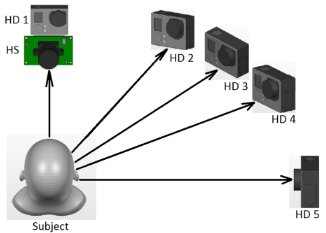
\includegraphics[width=0.6\columnwidth]{fig/ouluMultiView.jpg}
    \caption{Illustration of the multi-view setup used in the OuluVS2 recording, reference to figure???}
    \label{fig:ouluMultiView}
\end{figure}
\begin{figure}[h]
    \centering
    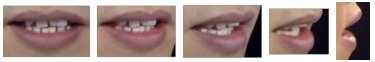
\includegraphics[width=\columnwidth]{fig/ouluPreprocessed.jpg}
    \caption{Example of the preprocessed data with with the region of interest.}
    \label{fig:ouluPreprocessed}
\end{figure}

\begin{table}[h]
    \begin{tabular}{l|p{6.2cm}}
        \multirow{2}{*}{(1) Digits}  
        & "1 7 3 5 1 6 2 6 6 7"\\
        & "4 0 2 9 1 8 5 9 0 4"\\
        \hline
        \multirow{2}{*}{(2) Phrases}  
        & "Thank you"\\
        & "Have a good time"\\
        \hline
        (3) TIMIT & "Chocolate and roses never fail as a romantic gift"
    \end{tabular}
    \caption{Examples of the three different scenarios used}
    \label{tab:ouluSecnarioExamp}
\end{table}

\section{Method}
\label{sec:method}

In this section our approach to solve the Automatic Lip-reading is presented.
The high-level architecture is first introduced, where the main components and their functions is described.
The particular architectures which we like to evaluate is then presented.

\subsection{High-level Architecture}
In figure \ref{fig:highLevelArchitecture} an illustration of the high-level architecture can be seen with the three main components; \textit{Visual model}, \textit{temporal model} and classifier.
In the figure the flow of information can also be seen, from the sequence of images inputted to the architecture and to the outputted class probabilities. 
%For this project the \textit{input} data consist of a sequence of images, where the dataset presented in section \ref{sec:dataset} is used the extracted region-of-interest.
The \textit{visual model} is used to extract features from the input image.
These features is then passed on to the \textit{temporal model} where they are correlated in time.
The time correlated features is then inputted to the classifier which is outputting the different class probabilities.
For each of the three main components, different implementations is of interest where each of these is listed in figure \ref{fig:highLevelArchitecture}. 
Each of the different methods is presented in the following sections.
\begin{figure}[h]
    \centering
    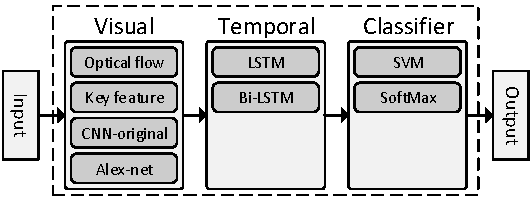
\includegraphics[width=\columnwidth]{fig/highLevelArchitecture.pdf}
    \caption{High-level architecture used}
    \label{fig:highLevelArchitecture}
\end{figure}

\subsection{Visual Model}
For the feature extraction 4 different methods is of interest, where two of these make use of neural network's and the other two is computer vision related.
\paragraph{CNN-original}
This visual model is corresponding to the one used in the state-of-the-art model, presented in \cite{Lee}.
An illustration of the model can be seen in figure \ref{fig:cnnOriginal}.
It make use of two convolutional layers with 16 to 256 filters in the shape of (3,3).
Each convolutional layer has a successive max-pooling layer in the shape of (2,2).
Lastly a fully connected layer with a dimension of 8 to 64 outputs is used.
\begin{figure}[h]
    \centering
    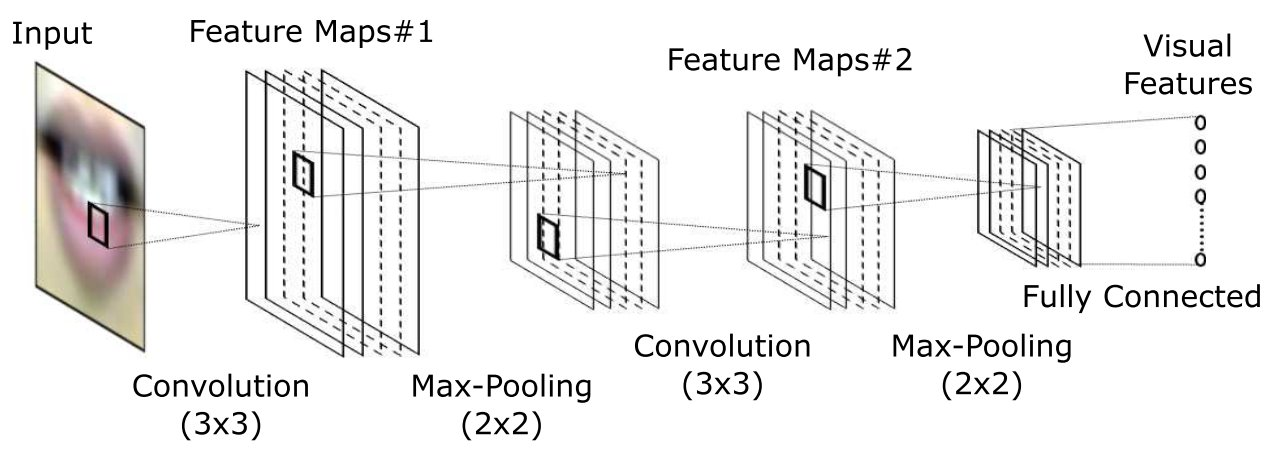
\includegraphics[width=\columnwidth]{fig/cnnOriginal.jpg}
    \caption{CNN-original}
    \label{fig:cnnOriginal}
\end{figure}

\paragraph{Alex-Net}
A popular neural network architecture for image recognition is an Alex-net\cite{Krizhevsky2012}.
This architecture is a deep CNN as depicted in figure \ref{fig:alexNet}.
\begin{figure}[h]
    \centering
    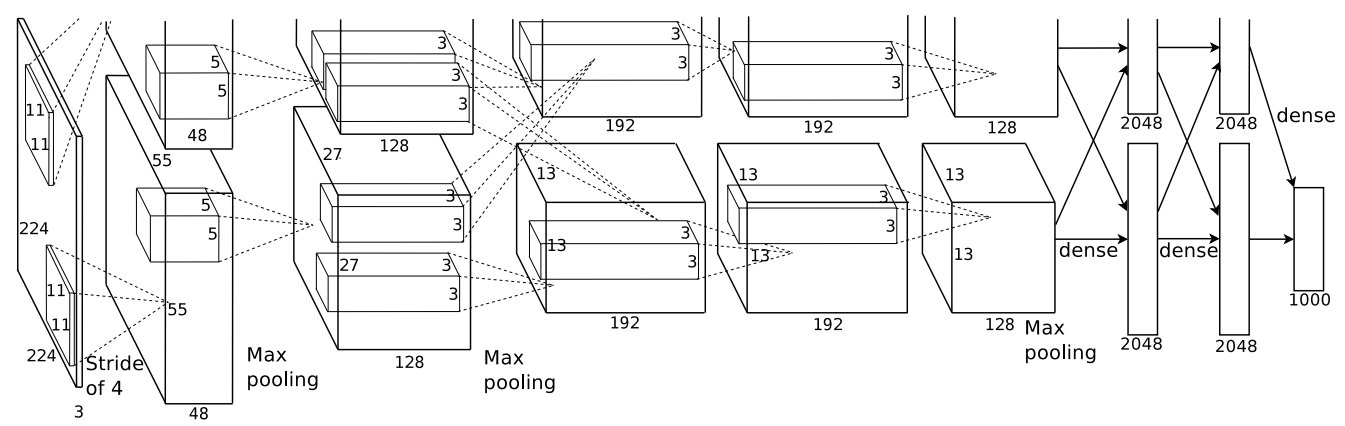
\includegraphics[width=\columnwidth]{fig/alexNet.jpg}
    \caption{Alex-net}
    \label{fig:alexNet}
\end{figure}

\paragraph{Optical flow}
For the calculation of optical flow we expect the differential method commonly denoted as the Lucas-Kanade method\cite{Lucas1981}.
The method have the assumption of the flow begin essentially constant in a local neighbourhood.

\paragraph{Key features}
For the key feature extraction a method similar to the one presented in \cite{Li2008} is used.
The mouth is divided in to four parts, lower and upper part of the upper lip and lower and upper part of the lower lip.
A vertical grid is then made, where the coordinates of the intersection points is used.
An illustration of this can be seen in figure \ref{fig:keyFeature}.
\begin{figure}[h]
    \centering
    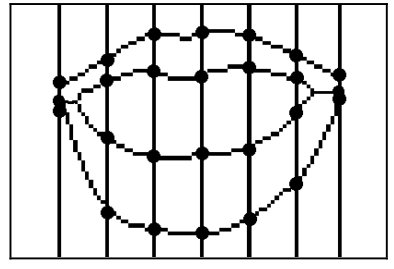
\includegraphics[width=0.5\columnwidth]{fig/keyFeature.jpg}
    \caption{Key Feature}
    \label{fig:keyFeature}
\end{figure}

\subsection{Temporal model}
Two different temporal models is used, which is \textit{LSTM} and \textit{bidirectional-LSTM}.
For both of these models a two layered design is used, where the size of each layer is here varying with the number of output features from the visual model.

\subsection{Classifier}
For the classification two different methods is evaluated, namely a support vector machine (SVM) and softmax.

%\subsection{Proposed Architecture}
%We propose to use several different model for both the visual and temporal model.
%We will here implement and evaluate each of these models to see how they perform and compare this to the current state-of-the-art architecture.
%We will here use the visual and temporal models listed in table \ref{tab:visualTemporalModel}.

%\begin{table}
%\centering
%\begin{tabular}{l|l}
%Visual Model & Temporal Model\\
%\hline
%CNN-original & LSTM\\
%Alex-net & B-LSTM\\
%Optical Flow & \\
%Key Features &
%\end{tabular}
%\caption{Table with the different Visual and Temporal models used}
%\label{tab:visualTemporalModel}
%\end{table}

%From these visual and temporal models a total of 10 different architectures can be obtained by combining a single visual model with a single temporal model.
%These 10 single model architectures is all listed in table \ref{tab:singleModelArc}.
%Beside these single model architecture further can be obtained by combining multiple visual models with a single temporal model.
%Before combining multiple visual models, we first propose to evaluate the performance of the single model architectures.
%
%
%In our approach we will first obtain results from the 10 basic models and then 
%
%
%Temporal Model
%LSTM
%B-LSTM
%
%
%Alex-net + LSTM
%CNN-original + Bidirectional LSTM
%Optical flow + LSTM
%Key features + LSTM

\section{Experiment and Result}


\subsection{Single-view Lip-Reading}

\begin{figure}[h]
	\centering
	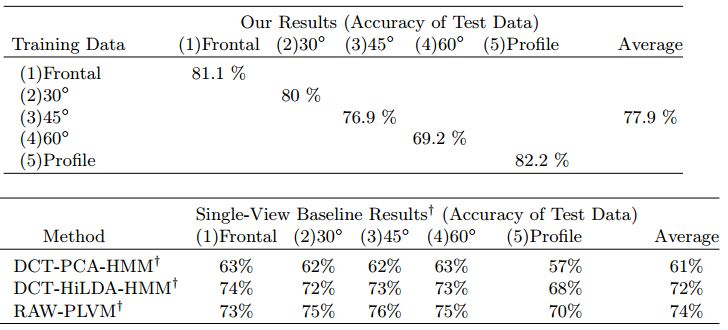
\includegraphics[width=\columnwidth]{fig/s1.jpg}
	\caption{Single-view test accuray of word phrases.}
	\label{fig:s1}
\end{figure}
Fig \ref{fig:s1} shows the accuracy result of single - view on word phrase test data. The results are similar with our previous paper \cite{Lee}. We have best accuracy on Profile view.

\begin{figure}[h]
	\centering
	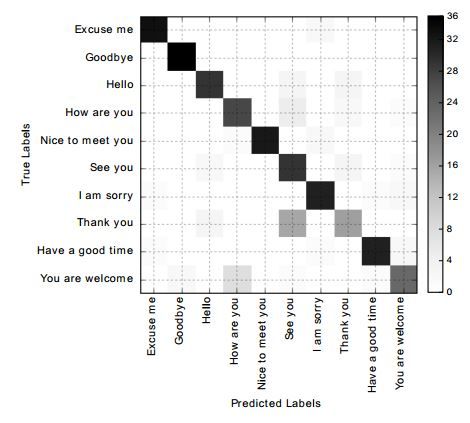
\includegraphics[width=\columnwidth]{fig/s2.jpg}
	\caption{Confusion matrix of best of Single Views}
	\label{fig:s2}
\end{figure}
Fig \ref{fig:s2} is Confusion matrix of profile view, which is the best in single view test accuracy. The x-axis is prediction classes and the y-axis is true classes.
We can see that 'Thank you' and 'See you' is the most confusing word phrase.


\subsection{Cross-view Lip-Reading}
In Cross view experiment, we conduct it as two seperate stages. At first stage, as we refer it to 'Cross View(CV)', we train 5 total view data all together simultaneously and test each view seperately.  In this approach, we get the
average accuracy 82.6\%, and all of the results are better than preliminary results.
 At Second stage, we call this stage as "Cross-view2(CV2)", and here, we finetune the first stage result to a certain view and also test with the certain view. Here, we can see slightly better performance on each view and also on average compare to CV.
  
\begin{figure}[h]
	\centering
	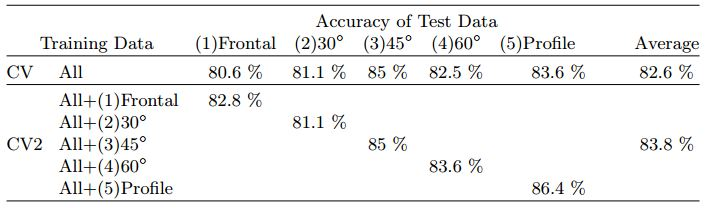
\includegraphics[width=\columnwidth]{fig/c1.jpg}
	\caption{Cross-view test accuracy. CV : Cross View, CV2 : Cross View 2}
	\label{fig:c1}
\end{figure}
In CV, Profile view shows the best performance(83.6\%), and in CV2, 60-degree view shows the best performance on total Cross view experiment.

\begin{figure}[h]
	\centering
	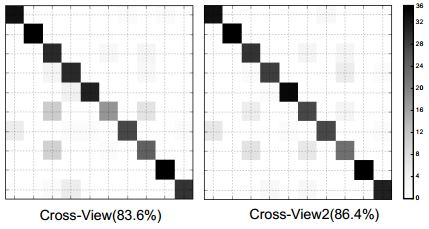
\includegraphics[width=\columnwidth]{fig/c2.jpg}
	\caption{Confusion matrices of best of  Cross Views}
	\label{fig:c2}
\end{figure}
The confusion matrices of test accuracies of profile view(CV) and 60-degree view (CV2). The axis lable share the same label in fig \ref{fig:s2}. It shows that
a gradual improvement from single-view to cross-view.  

\subsection{Multi-view Lip-Reading}
In Multi-view experiment, we conduct slightly different type of architecture as inputs are five times larger then single or cross view experimetn. Here, we conduct Merge Image method as this method of multi-view is best in our previous paper.

\subsubsection*{Merge Images}
\begin{figure}[h]
	\centering
	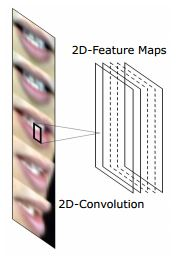
\includegraphics[width=0.4\columnwidth]{fig/mi.jpg}
	\caption{Merge Image model architencture for the multi-view setting}
	\label{fig:mi}
\end{figure}
As shown in fig \ref{fig:mi}, we append five images from the different
view at the same time into a single image as an input of the visual model. In this
architecture, we expect to learn all the five view feature by 2D-CNN. While out
of our experiment, a more elaborate configuration is that all five images avoid
convolving each other along the edges.

Despite it has more feature (give times more inputs), the result is worse than cross-view.
Fig \ref{fig:summary} shows the summary of all experiment through this paper.
\begin{figure}[h]
	\centering
	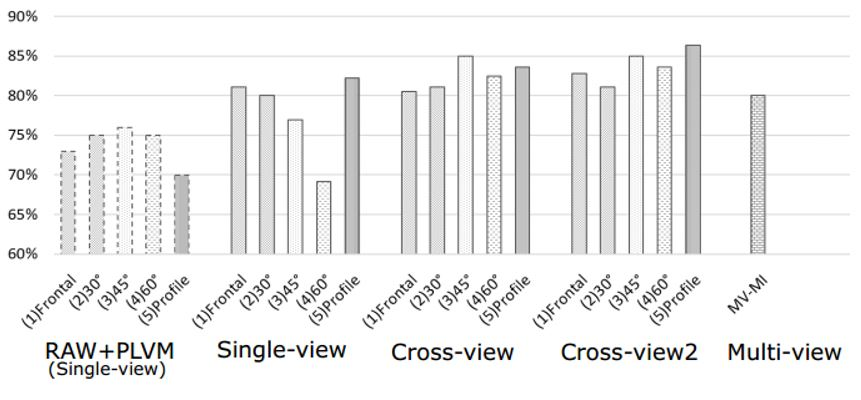
\includegraphics[width=\columnwidth]{fig/summary.jpg}
	\caption{The summary of the accuraciese. MV-MI is refers to Merge Images.}
	\label{fig:summary}
\end{figure}
\section{Conclusion}
The conclusion goes here.


\bibliographystyle{IEEEtran}
 %argument is your BibTeX string definitions and bibliography database(s)
\bibliography{tmp,mendeley}

% An example of a floating figure using the graphicx package.
% Note that \label must occur AFTER (or within) \caption.
% For figures, \caption should occur after the \includegraphics.
% Note that IEEEtran v1.7 and later has special internal code that
% is designed to preserve the operation of \label within \caption
% even when the captionsoff option is in effect. However, because
% of issues like this, it may be the safest practice to put all your
% \label just after \caption rather than within \caption{}.
%
% Reminder: the "draftcls" or "draftclsnofoot", not "draft", class
% option should be used if it is desired that the figures are to be
% displayed while in draft mode.
%
%\begin{figure}[!t]
%\centering
%\includegraphics[width=2.5in]{myfigure}
% where an .eps filename suffix will be assumed under latex, 
% and a .pdf suffix will be assumed for pdflatex; or what has been declared
% via \DeclareGraphicsExtensions.
%\caption{Simulation results for the network.}
%\label{fig_sim}
%\end{figure}

% Note that the IEEE typically puts floats only at the top, even when this
% results in a large percentage of a column being occupied by floats.


% An example of a double column floating figure using two subfigures.
% (The subfig.sty package must be loaded for this to work.)
% The subfigure \label commands are set within each subfloat command,
% and the \label for the overall figure must come after \caption.
% \hfil is used as a separator to get equal spacing.
% Watch out that the combined width of all the subfigures on a 
% line do not exceed the text width or a line break will occur.
%
%\begin{figure*}[!t]
%\centering
%\subfloat[Case I]{\includegraphics[width=2.5in]{box}%
%\label{fig_first_case}}
%\hfil
%\subfloat[Case II]{\includegraphics[width=2.5in]{box}%
%\label{fig_second_case}}
%\caption{Simulation results for the network.}
%\label{fig_sim}
%\end{figure*}
%
% Note that often IEEE papers with subfigures do not employ subfigure
% captions (using the optional argument to \subfloat[]), but instead will
% reference/describe all of them (a), (b), etc., within the main caption.
% Be aware that for subfig.sty to generate the (a), (b), etc., subfigure
% labels, the optional argument to \subfloat must be present. If a
% subcaption is not desired, just leave its contents blank,
% e.g., \subfloat[].


% An example of a floating table. Note that, for IEEE style tables, the
% \caption command should come BEFORE the table and, given that table
% captions serve much like titles, are usually capitalized except for words
% such as a, an, and, as, at, but, by, for, in, nor, of, on, or, the, to
% and up, which are usually not capitalized unless they are the first or
% last word of the caption. Table text will default to \footnotesize as
% the IEEE normally uses this smaller font for tables.
% The \label must come after \caption as always.
%
%\begin{table}[!t]
%% increase table row spacing, adjust to taste
%\renewcommand{\arraystretch}{1.3}
% if using array.sty, it might be a good idea to tweak the value of
% \extrarowheight as needed to properly center the text within the cells
%\caption{An Example of a Table}
%\label{table_example}
%\centering
%% Some packages, such as MDW tools, offer better commands for making tables
%% than the plain LaTeX2e tabular which is used here.
%\begin{tabular}{|c||c|}
%\hline
%One & Two\\
%\hline
%Three & Four\\
%\hline
%\end{tabular}
%\end{table}


% Note that the IEEE does not put floats in the very first column
% - or typically anywhere on the first page for that matter. Also,
% in-text middle ("here") positioning is typically not used, but it
% is allowed and encouraged for Computer Society conferences (but
% not Computer Society journals). Most IEEE journals/conferences use
% top floats exclusively. 
% Note that, LaTeX2e, unlike IEEE journals/conferences, places
% footnotes above bottom floats. This can be corrected via the
% \fnbelowfloat command of the stfloats package.











% trigger a \newpage just before the given reference
% number - used to balance the columns on the last page
% adjust value as needed - may need to be readjusted if
% the document is modified later
%\IEEEtriggeratref{8}
% The "triggered" command can be changed if desired:
%\IEEEtriggercmd{\enlargethispage{-5in}}

% references section

% can use a bibliography generated by BibTeX as a .bbl file
% BibTeX documentation can be easily obtained at:
% http://mirror.ctan.org/biblio/bibtex/contrib/doc/
% The IEEEtran BibTeX style support page is at:
% http://www.michaelshell.org/tex/ieeetran/bibtex/
%\bibliographystyle{IEEEtran}
% argument is your BibTeX string definitions and bibliography database(s)
%\bibliography{IEEEabrv,../bib/paper}
%
% <OR> manually copy in the resultant .bbl file
% set second argument of \begin to the number of references
% (used to reserve space for the reference number labels box)

%\begin{thebibliography}{1}
%
%\bibitem{IEEEhowto:kopka}
%H.~Kopka and P.~W. Daly, \emph{A Guide to \LaTeX}, 3rd~ed.\hskip 1em plus
%  0.5em minus 0.4em\relax Harlow, England: Addison-Wesley, 1999.
%
%\end{thebibliography}




% that's all folks
\end{document}


